\documentclass{article}
\usepackage{amsmath, amssymb, amsfonts}
\usepackage{fullpage}
\usepackage{enumerate}
\usepackage[linesnumbered,ruled,vlined]{algorithm2e}
\usepackage{hyperref}
\usepackage{graphicx}
\usepackage{comment}

\title{CS 4780/5780 Homework 8\vspace{-10pt}}
\author{Due: Thursday 29/11/18 11:55pm on Gradescope}
\date{}

\begin{document}
    \maketitle
	\section*{Problem 1:  Regression Trees}
	\begin{enumerate}
	\item[(a)] You are given a dataset $D=\{(-3, -20), (-2, -20), (-1, -17), (0, 15), (1, 25), (2, 26)\}$ and you want to build a regression tree for this dataset. Recall that the impurity for the regression tree model is  defined as
	$$
	L(S) = \frac{1}{|S|}\sum_{(x_i, y_i)\in S}(y_i - \bar{y}_S)^2,
	$$
	where $\bar{y}_S = \frac{1}{|S|}\sum_{(x_i, y_i)\in S}y_i$. Draw the regression tree $T_0$ built by the ID3-Algorithm which was introduced in class.(There are multiple correct thresholds. Choose one of them to draw.)
	
	\item[(b)] We keep the definition of $L(S)$ as (a). Prove that $L(S) \geq \frac{|S_1|}{|S|}L(S_1) + \frac{|S_2|}{|S|}L(S_2)$, where $S_1 \cup S_2 = S$ and $S_1\cap S_2 = \emptyset$. This conclusion tells us the impurity of a regression tree never increases after one split.
	
	\begin{comment}
	\item[b] 
	\begin{figure}
	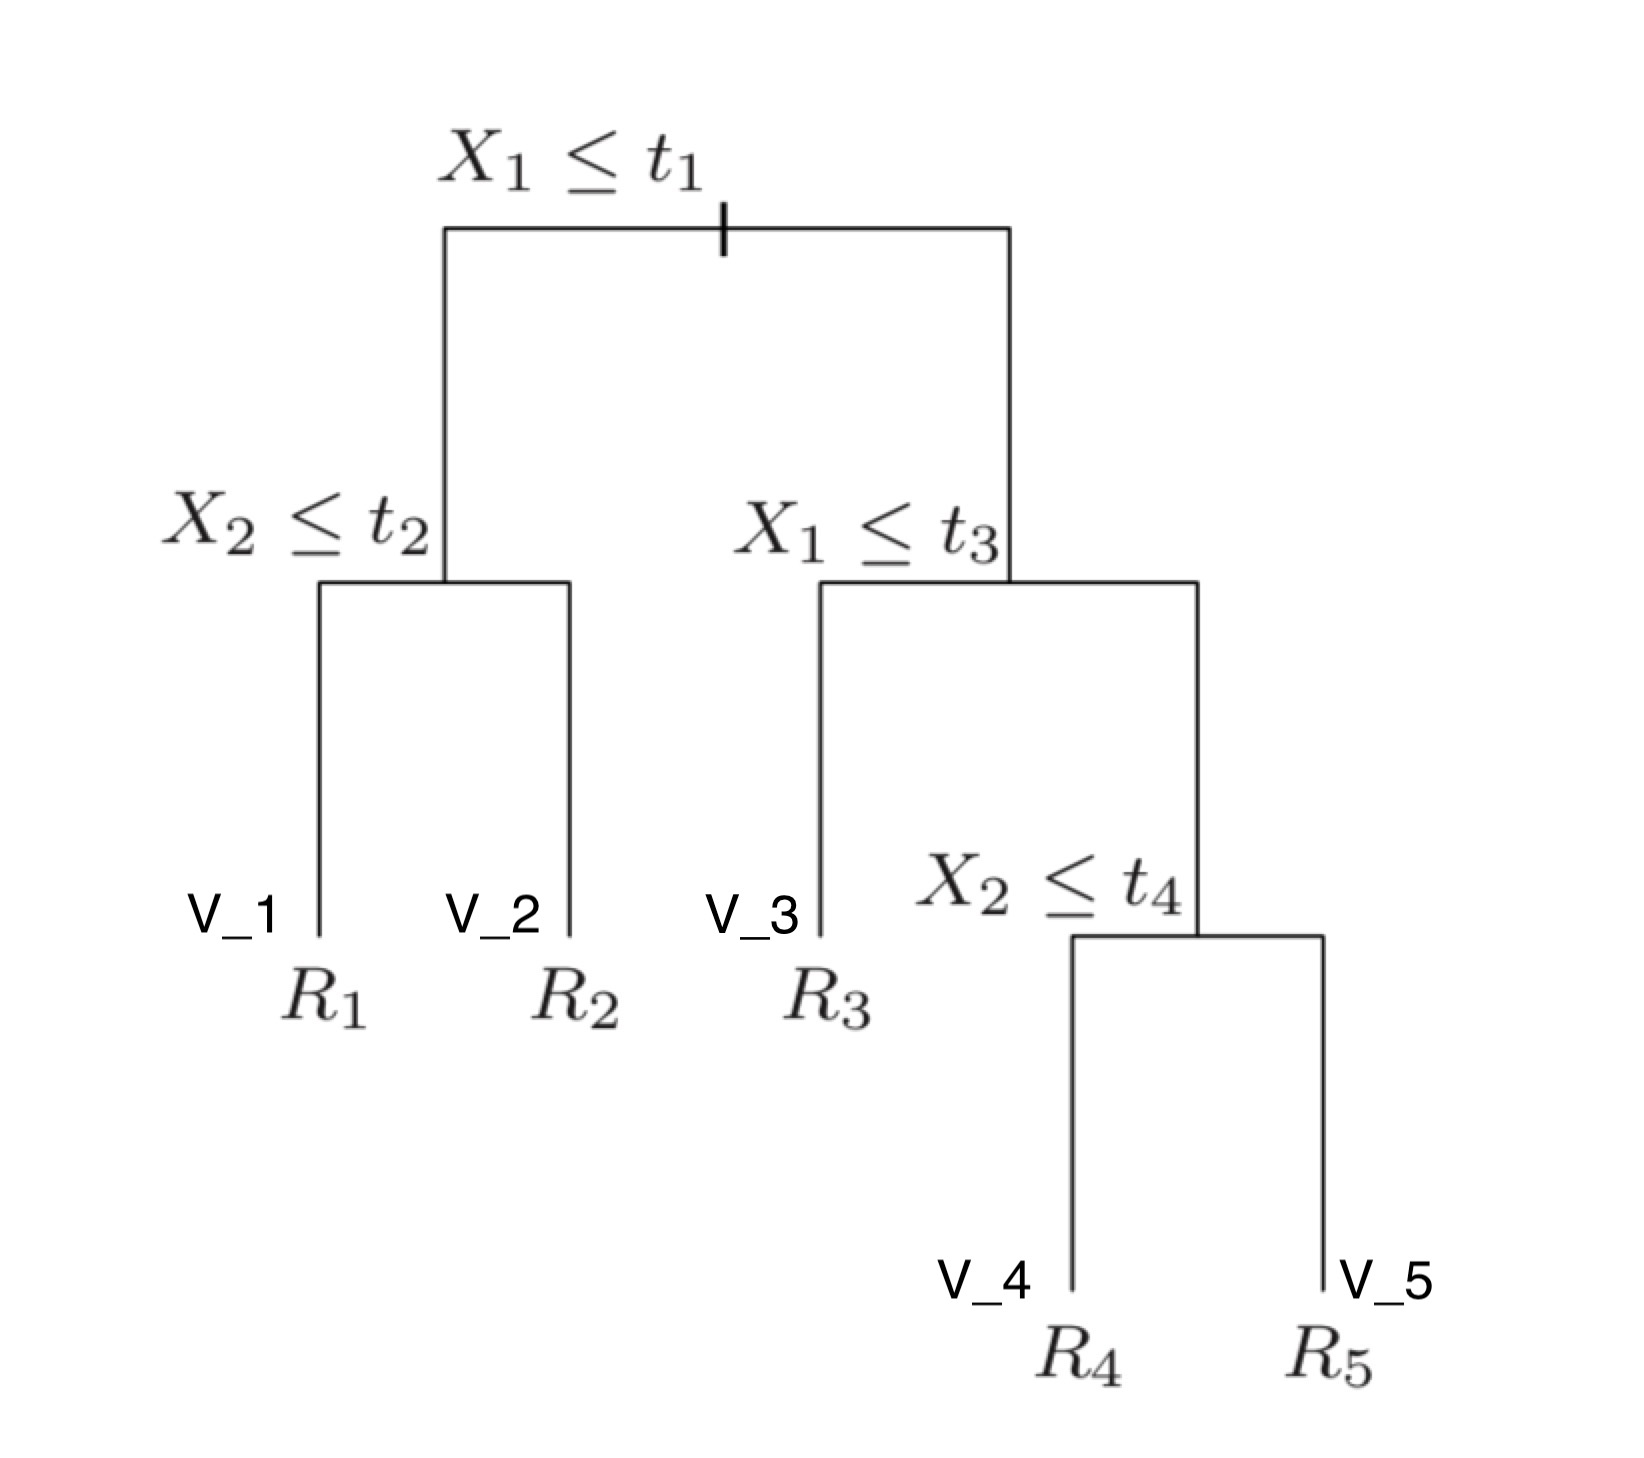
\includegraphics[scale=0.15]{T1}
	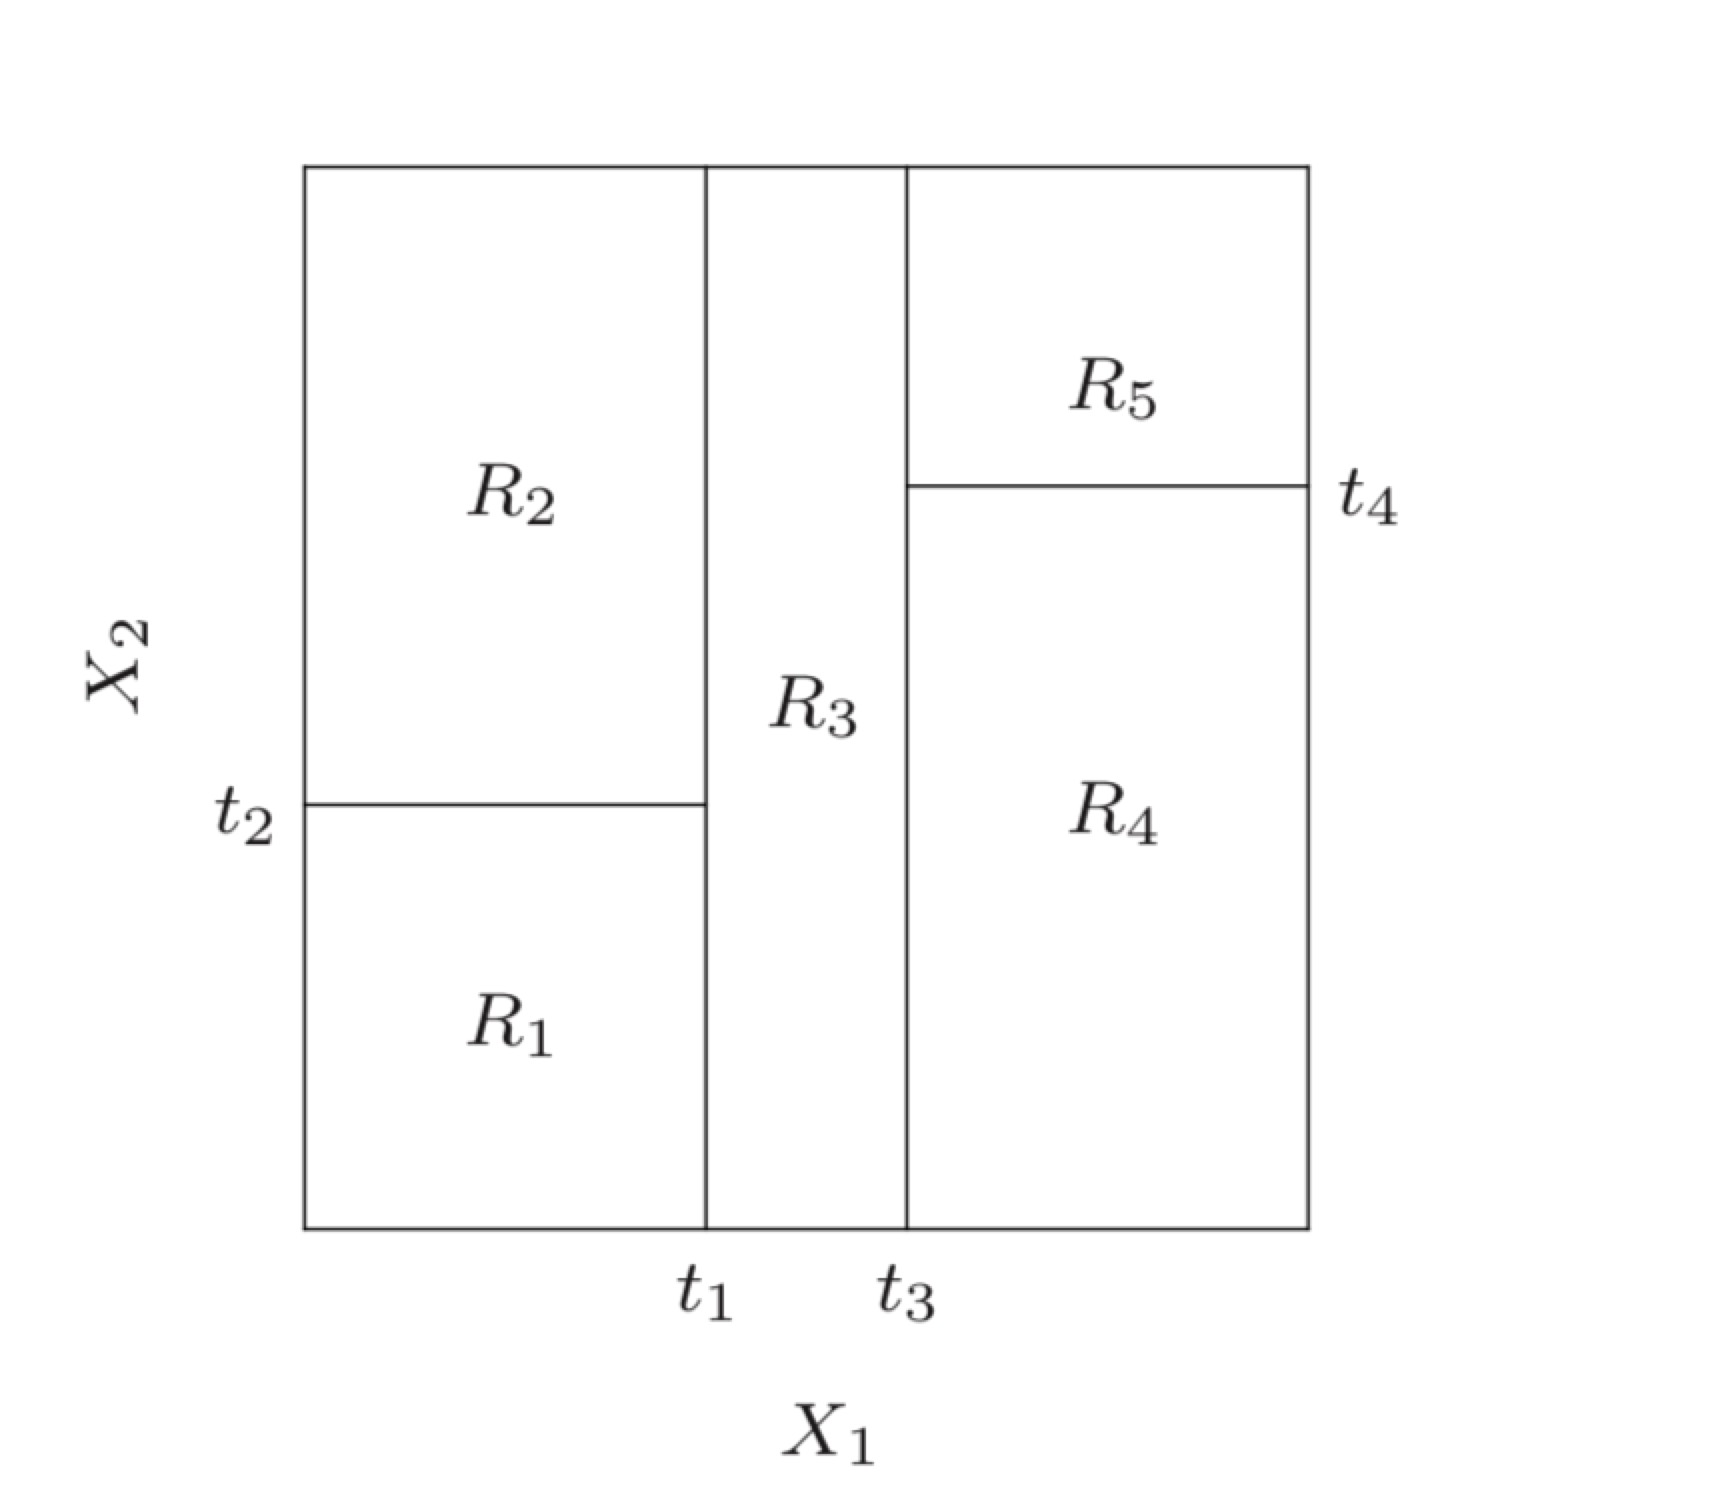
\includegraphics[scale=0.15]{T2}
	\caption{An example for Regression Tree}
	\label{fig_rt}
	\end{figure}
	\begin{figure}
	\centering
	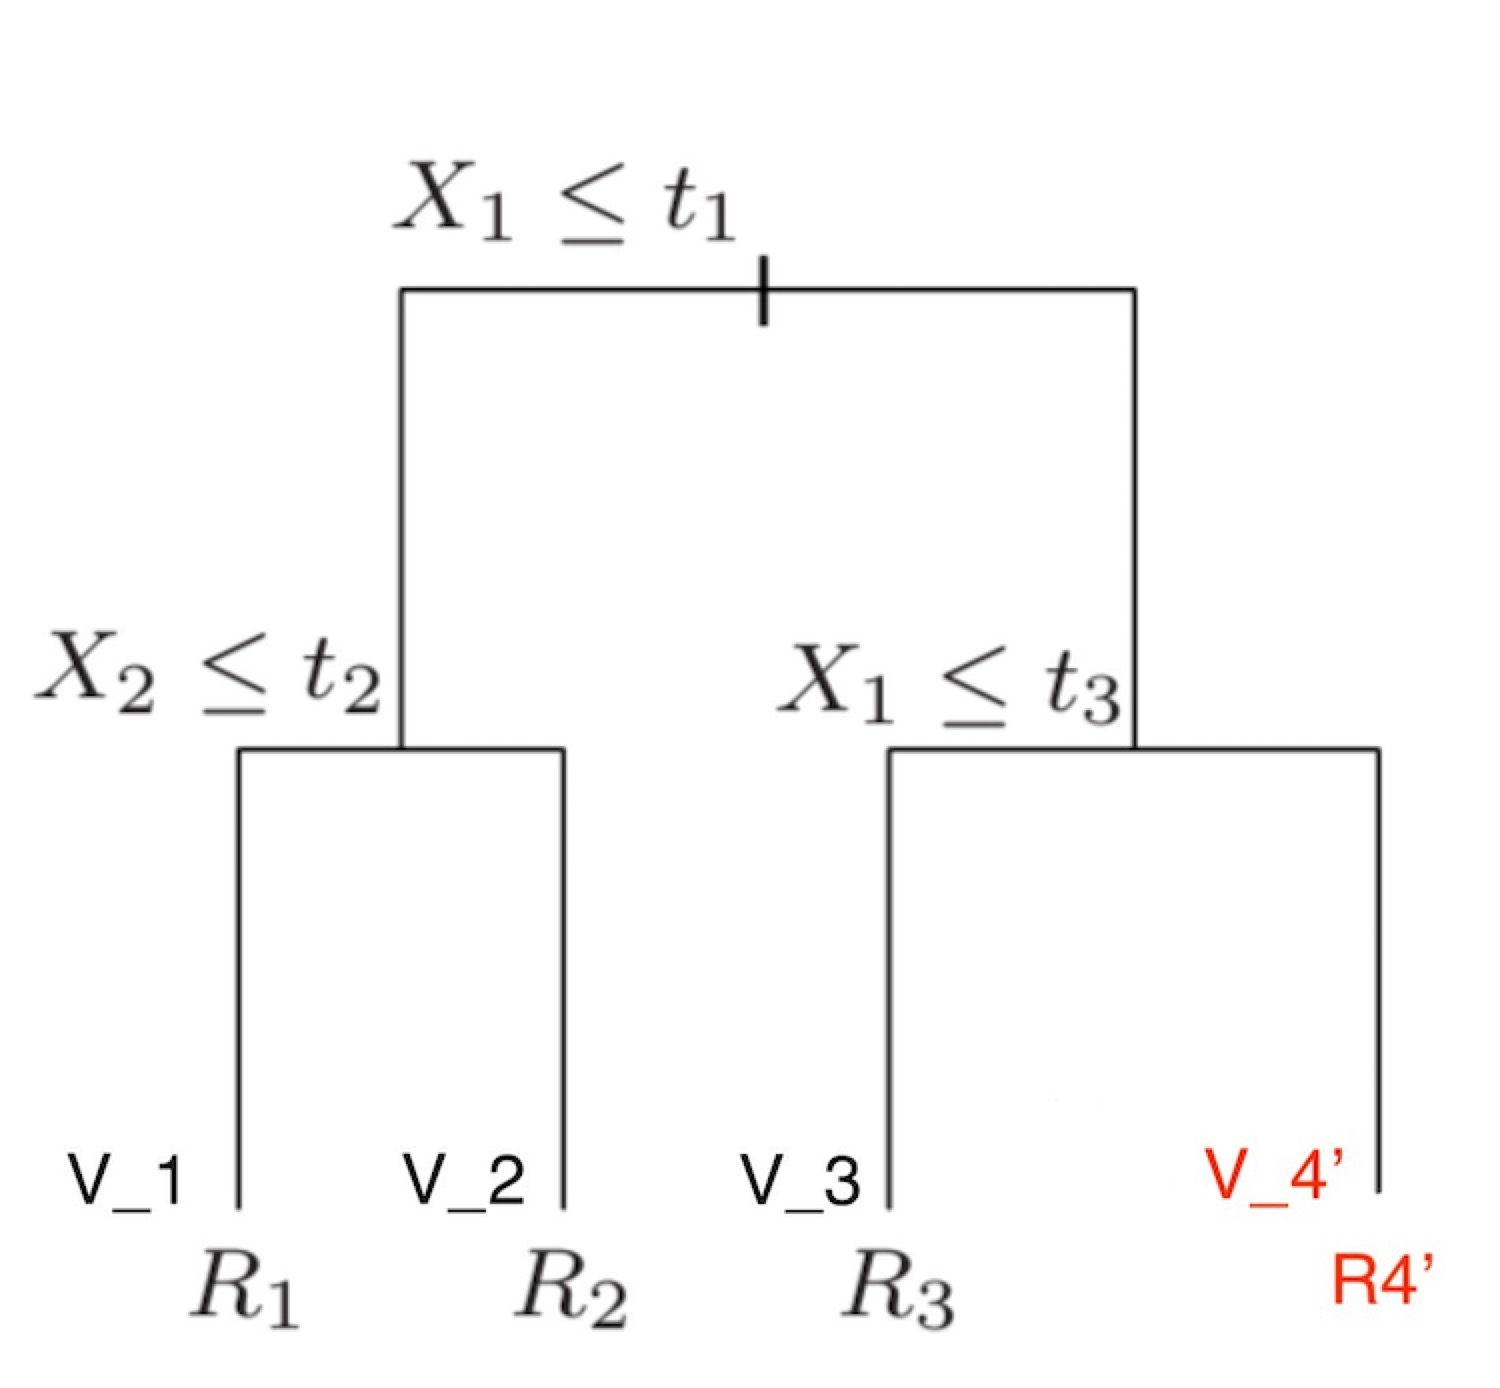
\includegraphics[scale=0.15]{T3}
	\caption{An example for Subtree}
	\label{fig_sbrt}
	\end{figure}
	\textbf{Notation.} Let us first introduce some notation for a regress tree $T$ (See Figure \ref{fig_rt}):
	\begin{itemize}
	\item Terminal node $V_m$: the $m^{th}$ node we stop to split.
	\item Region $R_m$: the region of $x$ defined by the path from root to terminal node $V_m$.
	\item $|T|$: the number of leaf nodes in the tree $T$.
	\item $N_m$: $|\{(x, y)\in D: x\in R_m\}|$.
	\item $L_m(T)$: is the impurity of $\{(x, y)\in D: x\in R_m\}$.
	\item Subtree $T'$: a subtree $T' \subseteq T$ is any tree that can be obtained by pruning $T$, that is, collapsing any number of its internal (non-terminal) nodes. For example the tree in Figure \ref{fig_sbrt} is a subtree of the tree in Figure \ref{fig_sbrt}.
	\end{itemize}
	
	
	\textbf{Criterion.} One way to regulate the bias variance trade-off in regression trees is to limit the number of leaf nodes $|T|$. If $|T|=n$, the bias of a classifier will be $0$, but the variance will be very high. Conversely, if the number of leaf nodes is small, $|T|\ll n$, the tree will have low variance but suffer from high bias. 
	
	To find the right tradeoff between bias and variance, we define the cost complexity criterion for tree $T$:
	$$
	C_{\alpha}(T) = \sum_{m=1}^{|T|} N_mL_m(T) + \alpha |T|,
	$$
	where $\alpha\geq 0$ is the tuning parameter regulating the tradeoff between bias and variance. Note, this is very similar to regularization in empirical risk minimization. 
	
	We would like to find  $\min_T C_\alpha(T)$. One complication is that trees are myopic, that means sometimes splits do not decrease the loss, but increase $|T|$. Such splits strictly \emph{increase} $C_\alpha(T)$ but are necessary to get a low value at a later stage. So instead of optimization $C_\alpha$ directly, a common strategy is to first build a full tree $T_0$ (which minimizes $C_0$) and then prune it back to optimize $C_\alpha$ for some given $\alpha>0$. 


	\textbf{Weakest Link.} The \textit{weakest link} pruning procedure is one effective strategy to prune a tree:
	\begin{itemize}
	\item successively collapse the internal node that produces the smallest per-node increase in $\sum_{m=1}^{|T|} N_mL_m(T) $.
	\item continue until we produce the single-node (root) tree.
	\end{itemize}
	
	\textbf{Existed Results. }You can use the following results directly without proof: for each $\alpha$, there is a unique smallest subtree $T_{\alpha}\subseteq T_0$ that minimizes $C_{\alpha}(T)$. Moreover, the sequence of subtrees obtained by pruning under the \textit{weakest link}, must contain $T_{\alpha}$.
	
	\textbf{Problem. }Please find the $T_\alpha\subseteq T_0$ with $\alpha = \frac{1}{2}$, where the tree $T_0$ is what you computed in (a). 
	\end{comment}
	
	\end{enumerate}
	
	%\section*{Problem 2:  Ensemble of Independent Models}
	%Given a dataset $D = \{(x_i, y_i)\mid i=1, \cdots, n\}$ where $y_i \in \{+1, -1\}$, you are going to do a classification task by an ensemble model $H$. More specifically,  you are given $2k + 1$ independent models $H_1, H_2, \cdots, H_{2k + 1}$. Each model $H_j$ has probability $p_i$ to make the correct prediction for data $(x_i, y_i)$. We further assume that for each model $H_j$, the predictions for different data are independent. Then $E[\sum_{i=1}^n I[H_j(x_i) = y_i]] = \sum_{i=1}^n p_i$. The ensemble model $H$ is defined as follow:
	%$$
	%H(x_i) =
	%\left\{
	%\begin{array}{rcl}
	%1      &      & {  |\{j\mid H_{j}(x_i) = 1\}| > |\{j\mid H_{j}(x_i) = 0\}| }\\
	%0     &      & { |\{j\mid H_{j}(x_i) = 1\}| < |\{j\mid H_{j}(x_i) = 0\}| }
	%\end{array} \right.
	%$$
	%Prove that $E[\sum_{i=1}^n I[H(x_i) = y_i]] = \sum_{i=1}^n p_i$.
	
	\section*{Problem 2: Normalization Update in Adaboost}
	In the Adaboost, we keep $\sum_{i=1}^n w^i_t = 1$. In the iteration $t$ of the algorithm, we update $w_t^i$ as follow: 
	$$w^i _{t+1}\leftarrow \frac{w^i_t\cdot e^{-\alpha_{t+1} h_{t+1}(x_i)y_i}}{2\sqrt{\epsilon_{t+1}(1-\epsilon_{t+1})}}$$
	where $\alpha_{t+1} = \frac{1}{2}\log \left(\frac{1 - \epsilon_{t+1}}{\epsilon_{t+1}}\right)$ and  $\epsilon_{t+1} = \sum_{i:h_{t+1}(x_i)\neq y_i}w^i_t$. Prove that if $\sum_{i=1}^n w^i_t = 1$, $\sum_{i=1}^n w^i_{t+1} = 1$, i.e. $\sum_{i=1}^{n} w^i_t \cdot e^{-\alpha_{t+1} h_{t+1}(x_i)y_i} = 2\sqrt{\epsilon_{t+1} (1-\epsilon_{t+1})}$. (Remember in the Adaboost, $h_{t+1}(x_i),y_i\in \{+1, -1\}$.)
	

\end{document}